\chapter{Future Work}
\label{ch:Future}
%\chaptertoc
\noindent

% Future works can go toward two branches: theory side with the performance model and the other branch with proactive load balancing.
% - Performance model:
% 		+ Tasks with dependencies, how efficient if some of them are migrated
%			+ System with heterogenous distributed memory system, leading to different communication overhead when migrating tasks
%			+ Estimating the bound with probability
%	- Further proactive LB:
%			+ How can we automate load prediction models or build a generative prediction mode?
%			+ How can we build a scheme for auto-feeding as well as auto-training the load prediction models at runtime?
%			+ The proactive scheme can merge other usefull information from communication side, e.g., topology information, ... This can generate a better selection algorithm for task migration.
%			+ Porting the idea of scheduling tasks across multiple applications for real use cases in HPC

This chapter introduces potential works in the future as extensions from the thesis. The proposed directions are mainly based on two branches: the first with our performance model and the second with a proactive load-balancing approach. We clarify and formulate these directions below. Figure \ref{fig:future_work_overview} shows an overview of potential directions in research based on this work. Our perspective highlights that we are on the shoulder of a giant regarding dynamic load balancing. A research direction is based on a chain of related works, and simultaneously it opens up new research questions that can be considered potential in the thesis. There are seven research questions addressed in the following paragraphs.\\

\begin{figure}[ht]
  \centering
  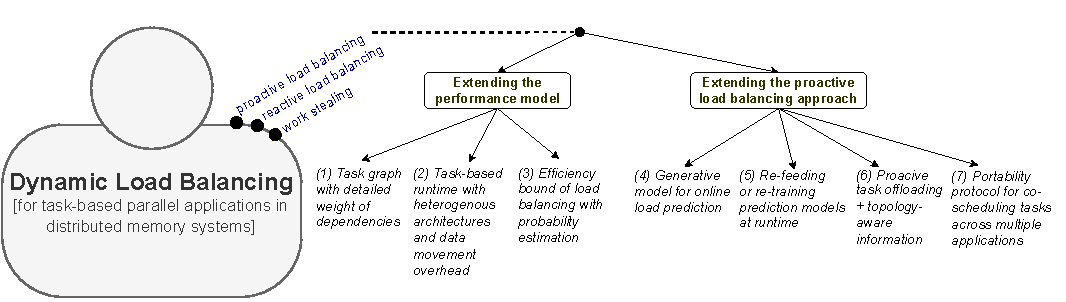
\includegraphics[scale=0.825]{./pictures/future_work/future_work_overview.pdf}
	\caption{An overview of future work for further research directions.}
	\label{fig:future_work_overview}
\end{figure}

% -------------------------------------------------
% Branch 1: theory side with a performance model
% -------------------------------------------------
First, the proposed performance model aims at work stealing and reactive load balancing under delay when migrating tasks. It revolves around the parameters of task distribution ($T$), the number of processes ($P$) with their execution speed ($S_{P}$) to indicate performance slowdown at some. $S_{P}$ can cause load imbalance, and the imbalance level is denoted by $R_{imb}$. Along with task migration delay time ($d$), we have built the model to estimate a bound of how many tasks can be migrated at a time. This model conducts an estimation of the efficiency bound for load-balancing approaches. Thereby, some research directions in the future can be oriented.

\begin{enumerate}[label=(\arabic*)]
	\item Task graph or task-based applications with dependencies. If we consider the edges in a graph represented for waiting time or weight between each other, then the research question is: how can we know the effect of these weights to task migration by work stealing, reactive or proactive balancing?
	\item System with heterogenous architectures and even they are distributed memory machines. The research question is: how can we formulate a model that shows different communication overhead in task migration?
	\item In general, a performance model can be relatively analyzed by probability. The question is: how can we better estimate the efficiency bound of load balancing?
\end{enumerate}

% -------------------------------------------------
% Branch 2: proactive load balancing
% -------------------------------------------------
Second, the proposed proactive load-balancing approach opens some further directions in the future. Its vision towards parallel applications can talk to each other. Our scheme dedicates one-core-off to control proactive load balancing, which can be considered as a communication channel for their talking. Moreover, we could force this core to perform asynchronous task characterization, ML-based load prediction, and proactive task offloading. Thereby, some research directions following this scheme can be addressed below.

\begin{enumerate}[label=(\arabic*)]
	\setcounter{enumi}{3}
	\item Regarding ML-based online load prediction, the challenge is: how can we build a generative model for predicting load automatically? This could help users perform machine learning models without prior configuration as well as prior knowledge.
	\item Following the previous idea, a following-up question can be raised: how can we extend the scheme for auto-feeding and auto-training these prediction models at runtime?
	\item Our proactive scheme can merge with other useful information on the communication side, e.g., topology information, real-time communication throughput, remote memory access, etc. This point can yield a question: how can we conduct a better selection algorithm for task migration at runtime?
	\item The portability direction of scheduling tasks across multiple applications is necessary for real use cases in HPC. We can aim at building a protocol for this idea. Our proposed question: how can we provide a new protocol in task-based parallel applications to enable scheduling tasks across multiple applications?
\end{enumerate}
